%%
%% Author: Thomas Schouten
%% 23-5-2018
%%

\documentclass[border=5mm, tikz]{standalone}

\usepackage{tikz}

\usetikzlibrary{positioning, arrows.meta}


% Default arrow length: (length right, length up)
\newcommand{\standardlength}{1,0}

% Default arrowhead.
\newcommand{\standardarrow}{-{Latex[length=2mm,width=2mm]}}

\newcommand{\standardbend}{30}


% Document
\begin{document}

    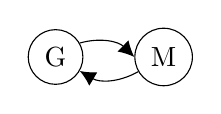
\begin{tikzpicture}[every node/.style={draw, circle}]
        \node (g) { G };
        \draw[\standardarrow] (g) to [bend left=\standardbend] ++(\standardlength)
        node[right] (m) { M };
        \draw[\standardarrow] (m) to [bend left=\standardbend] (g);
    \end{tikzpicture}

\end{document}